% PTCG agent architecture --- research-lane writeup.
% Build:  tectonic paper/architecture.tex      (or: pdflatex twice)
% No absolute paths, no external data files, no shell-escape. Fonts declared below.
\documentclass[11pt,a4paper]{article}

\usepackage[T1]{fontenc}
\usepackage[utf8]{inputenc}
\usepackage{lmodern}                 % declared font: Latin Modern (TeX Live base)
\usepackage[margin=25mm]{geometry}
\usepackage{amsmath,amssymb}
\usepackage{booktabs}
\usepackage{xcolor}
\usepackage{tikz}
\usepackage{pgfplots}
\usepackage{caption}
\usepackage[hidelinks]{hyperref}

\pgfplotsset{compat=1.16}
\usepgfplotslibrary{fillbetween}
\usetikzlibrary{positioning,arrows.meta,fit,backgrounds,calc}

\definecolor{cState}{RGB}{31,102,160}
\definecolor{cOpt}{RGB}{191,90,30}
\definecolor{cPad}{RGB}{150,150,150}
\definecolor{cV2}{RGB}{20,130,80}
\definecolor{cBad}{RGB}{170,30,40}

\newcommand{\srcfile}[1]{{\footnotesize\texttt{#1}}}
\newcommand{\tagM}{\textcolor{cV2}{\textsc{[measured]}}}
\newcommand{\tagT}{\textsc{[theorem]}}
\newcommand{\tagP}{\textsc{[practice]}}
\newcommand{\tagS}{\textcolor{cBad}{\textsc{[speculative]}}}
\newcommand{\tagU}{\textcolor{cBad}{\textsc{[unsourced]}}}

\title{\bfseries A Set-Transformer Agent for the Pok\'emon TCG:\\
Architecture, Evidence, and What Is Not Yet Justified}
\author{Research lane}
\date{2026-08-16}

\begin{document}
\maketitle

\begin{abstract}
\noindent
We describe the architecture of a set-transformer policy for the Pok\'emon Trading
Card Game competition, and --- deliberately given equal weight --- the boundary
between what its design choices are known to buy and what is currently asserted
without a measurement behind it. Three changes distinguish the current
architecture (v2) from its predecessor: a family-conditioned (FiLM) numeric
projection, multi-seed pooled attention with per-consumer read-outs, and
per-column input standardisation folded so that a warm start is exact. Each has
a stated mechanism; we check the mechanisms against the literature and against
the code, and we report one case where the project's own design document rejects
a component on evidence that does not support the rejection, and another where
two components are \emph{structurally inseparable} in the implementation and
therefore cannot be ablated as planned. We close with the measured
between-seed variation, which is the single most transferable result we have:
architecture differences of the size currently being reported sit close enough
to seed noise that single-run comparisons should not be published as findings.
\end{abstract}

\section{Evidence tags}

Every quantitative claim in this document carries one of five tags. A claim
without a traceable measurement does not appear.

\begin{center}
\begin{tabular}{ll}
\toprule
\tagT & follows by algebra or from a cited theorem \\
\tagP & established practice in the literature, not a theorem \\
\tagM & measured in this project, with the producing run named \\
\tagS & plausible mechanism, no measurement \\
\tagU & a number in circulation whose source could not be located \\
\bottomrule
\end{tabular}
\end{center}

\section{The token surface}

The game state is presented to the network as a \emph{set} of typed entity
tokens, not a sequence. State tokens and one token per legal option occupy a
single sequence, so all options are scored in one forward pass. Legality is a
property of the input: an illegal action is never constructed and therefore has
no logit.

\begin{figure}[h]
\centering
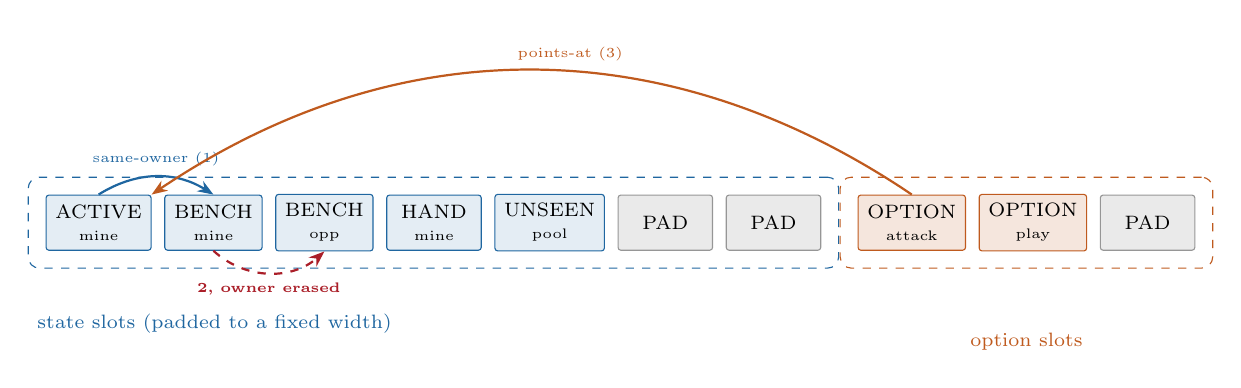
\begin{tikzpicture}[font=\small,node distance=1.6mm]
\tikzset{tok/.style={draw,rounded corners=1pt,minimum height=7mm,minimum width=12mm,align=center,font=\scriptsize}}
\node[tok,fill=cState!12,draw=cState] (s1) {ACTIVE\\\tiny mine};
\node[tok,fill=cState!12,draw=cState,right=of s1] (s2) {BENCH\\\tiny mine};
\node[tok,fill=cState!12,draw=cState,right=of s2] (s3) {BENCH\\\tiny opp};
\node[tok,fill=cState!12,draw=cState,right=of s3] (s4) {HAND\\\tiny mine};
\node[tok,fill=cState!12,draw=cState,right=of s4] (s5) {UNSEEN\\\tiny pool};
\node[tok,fill=cPad!20,draw=cPad,right=of s5] (p1) {PAD};
\node[tok,fill=cPad!20,draw=cPad,right=of p1] (p2) {PAD};
\node[tok,fill=cOpt!15,draw=cOpt,right=of p2,xshift=3mm] (o1) {OPTION\\\tiny attack};
\node[tok,fill=cOpt!15,draw=cOpt,right=of o1] (o2) {OPTION\\\tiny play};
\node[tok,fill=cPad!20,draw=cPad,right=of o2] (p3) {PAD};

\begin{scope}[on background layer]
\node[fit=(s1)(p2),draw=cState,dashed,inner sep=2.2mm,rounded corners] (sbox) {};
\node[fit=(o1)(p3),draw=cOpt,dashed,inner sep=2.2mm,rounded corners] (obox) {};
\end{scope}
\node[below=7mm of sbox.south west,anchor=west,font=\scriptsize,text=cState] {state slots (padded to a fixed width)};
\node[below=7mm of obox.south,font=\scriptsize,text=cOpt] {option slots};

\draw[-{Stealth[length=2mm]},cState,thick] (s1.north) to[bend left=32] node[above,font=\tiny,pos=0.5] {same-owner (1)} (s2.north);
\draw[-{Stealth[length=2mm]},cBad,thick,dashed] (s2.south) to[bend right=42] node[below,font=\tiny,pos=0.5] {\textbf{2, owner erased}} (s3.south);
\draw[-{Stealth[length=2mm]},cOpt,thick] (o1.north) to[bend right=34] node[above,font=\tiny,pos=0.45] {points-at (3)} (s1.north east);
\end{tikzpicture}
\caption{Token layout and typed relations. Relations are attribute-derived
(same-owner, same-zone, active-vs-active) or instance-specific (the
\texttt{option\_ptr} edge naming which state token an option refers to). The
dashed red edge is a defect, not a design: see \S\ref{sec:reldefect}.}
\label{fig:tokens}
\end{figure}

\paragraph{Padding is masked, and this is not a tuning choice. \tagT\ \tagM}
Unmasked attention places every \textsc{pad} slot in the softmax denominator, so
the representation of every \emph{real} token becomes a function of the padding
width --- a property of the batch, not of the game state. Training collates to a
state width of $160$; the serving featuriser pads to $192$. We held real token
content byte-identical and varied only the number of trailing \textsc{pad} slots,
using trained weights in evaluation mode:

\begin{center}
\begin{tabular}{lrr}
\toprule
& argmax changed, train $\to$ serve & mean $\max|\Delta \text{logit}|$ \\
\midrule
masked   & $0/300 = 0.00\%$          & $1.71\times10^{-6}$ \\
unmasked & $\mathbf{37/300 = 12.33\%}$ & $\mathbf{1.355}$ \\
\bottomrule
\end{tabular}
\end{center}

\noindent
The masked residual is floating-point kernel-tiling noise. The unmasked figure
means an unmasked model \emph{serves a different function than the one it
trained}. This also settles a separate claim: bucketing the pad width to
$\{64,96,160,232\}$ for a large serving speed-up is representationally free
\emph{under masking} and is not free without it.

\section{The numeric projection, and where FiLM enters}

\subsection{The defect being repaired}

Numeric columns are laid out per family, so the same column index carries
different quantities on different token families: column 8 is
\texttt{bench\_slot\_0} on a \textsc{bench} token and hand position $0$ on a
\textsc{hand} token. Permutation attribution of that single column, over 600
held-out frames, is $0.0241$ from \textsc{hand} against $0.0003$ from
\textsc{bench} and $0.0004$ from \textsc{active}. \tagM

In v1 the family enters the token representation \emph{additively}, after a
single shared linear map applied to all families.

\paragraph{An additive family embedding cannot modulate a linear map. \tagT}
Writing $z$ for the standardised numeric vector, $f$ for the family and $e(\cdot)$
for the additive embeddings,
\[
x_{\text{v1}} \;=\; e_{\text{fam}}(f) + e_{\text{own}}(o) + e_{\text{card}}(c) + Wz + b,
\qquad
\frac{\partial x_{\text{v1}}}{\partial z} \;=\; W ,
\]
which is independent of $f$. The family term shifts the output; it cannot change
how the map reads its input. The claim as stated in the project's design notes
is therefore correct.

\subsection{What FiLM does, exactly}

FiLM \cite{perez2018film} conditions a network on side information by a
feature-wise affine transform. In this implementation it is applied to the
\emph{input} of the projection, with per-family gain and offset vectors of the
same width as the numeric surface:
\[
x_{\text{v2}} \;=\; \dots + W\big(\gamma_f \odot z + \beta_f\big) + b,
\qquad
\frac{\partial x_{\text{v2}}}{\partial z} \;=\; W\,\mathrm{diag}(\gamma_f).
\]
So the contribution of column $j$ under family $f$ is $W_{:,j}\,\gamma_f[j]\,z_j$.

\begin{figure}[h]
\centering
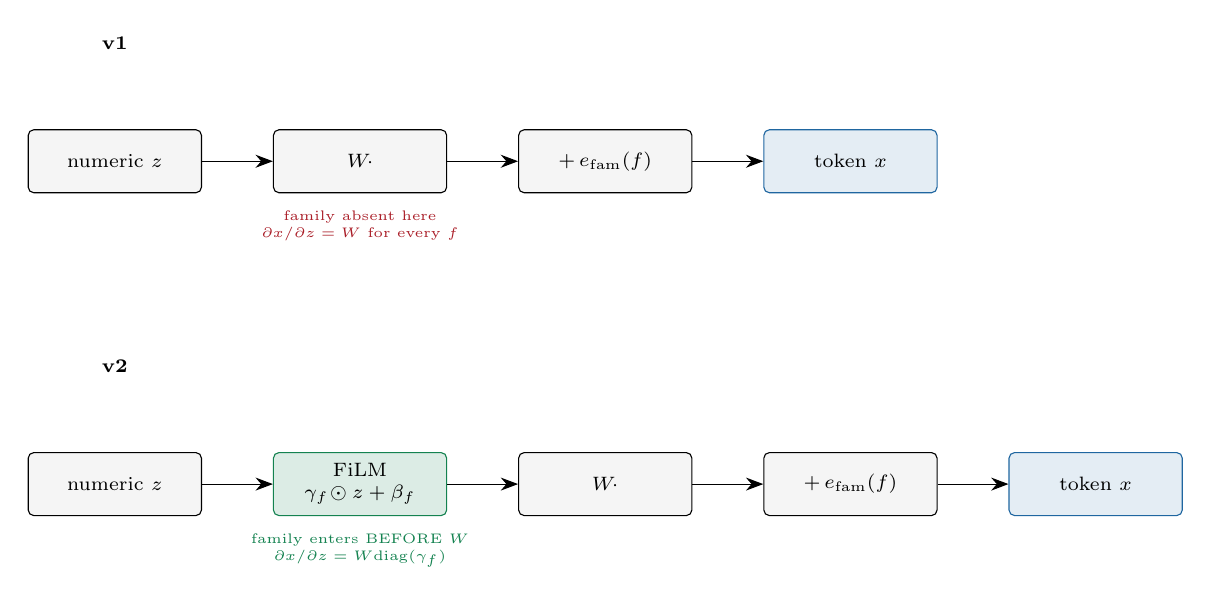
\begin{tikzpicture}[font=\small]
\tikzset{
  b/.style={draw,rounded corners=2pt,minimum height=8mm,minimum width=22mm,align=center,font=\scriptsize},
  ar/.style={-{Stealth[length=2.2mm]}}
}
% v1 path
\node[font=\scriptsize\bfseries] at (0,1.5) {v1};
\node[b,fill=black!4] (z1) at (0,0) {numeric $z$};
\node[b,fill=black!4,right=9mm of z1] (w1) {$W\!\cdot$};
\node[b,fill=black!4,right=9mm of w1] (a1) {$+\,e_{\text{fam}}(f)$};
\node[b,fill=cState!12,draw=cState,right=9mm of a1] (t1) {token $x$};
\draw[ar] (z1)--(w1); \draw[ar] (w1)--(a1); \draw[ar] (a1)--(t1);
\node[font=\tiny,text=cBad,below=1mm of w1,align=center] {family absent here\\$\partial x/\partial z=W$ for every $f$};

% v2 path
\node[font=\scriptsize\bfseries] at (0,-2.6) {v2};
\node[b,fill=black!4] (z2) at (0,-4.1) {numeric $z$};
\node[b,fill=cV2!15,draw=cV2,right=9mm of z2] (f2) {FiLM\\$\gamma_f\!\odot z+\beta_f$};
\node[b,fill=black!4,right=9mm of f2] (w2) {$W\!\cdot$};
\node[b,fill=black!4,right=9mm of w2] (a2) {$+\,e_{\text{fam}}(f)$};
\node[b,fill=cState!12,draw=cState,right=9mm of a2] (t2) {token $x$};
\draw[ar] (z2)--(f2); \draw[ar] (f2)--(w2); \draw[ar] (w2)--(a2); \draw[ar] (a2)--(t2);
\node[font=\tiny,text=cV2,below=1mm of f2,align=center] {family enters BEFORE $W$\\$\partial x/\partial z=W\mathrm{diag}(\gamma_f)$};
\end{tikzpicture}
\caption{Where family conditioning enters. In v1 the family is added after the
projection and cannot alter it. In v2 FiLM multiplies the projection's input, so
each (family, column) pair gets an independent scalar gain.}
\label{fig:film}
\end{figure}

\paragraph{The precise capability, and the precise limit. \tagT}
FiLM gives an \emph{independent scalar gain per (family, column)}. It can
therefore switch column 8 on for \textsc{hand} and off for \textsc{bench},
eliminating interference between two families that share a column index. It
cannot give column $j$ a different \emph{direction} in $\mathbb{R}^{d}$ per
family: that direction is $W_{:,j}$ for every family, and FiLM moves the
contribution only along the line $\mathrm{span}\{W_{:,j}\}$ (a negative gain
reverses it). Formally, FiLM is exactly the subfamily of per-family projections
constrained to $W_f = W\,\mathrm{diag}(\gamma_f)$.

\paragraph{Is FiLM the right instrument here? Yes, on the evidence that exists.}
The project's ground-up design document rejects FiLM, arguing that column 8 on
\textsc{hand} and on \textsc{bench} are ``unrelated quantities needing different
directions.'' The measurement offered in support ($0.0241$ versus $0.0003$) does
not show that. An attribution of $0.0003$ is a column the family does not use;
that is an \emph{interference} pattern, which a gate repairs, not a
\emph{direction conflict}, which a gate cannot. The rejection is stated more
strongly than its cited evidence supports. The cost argument favours FiLM
sharply: $2 \cdot N_{\text{fam}} \cdot w = 12{,}768$ parameters against
$N_{\text{fam}} \cdot d \cdot w \approx 2.45$M for per-family matrices, a factor
of roughly $192$. \tagM

\paragraph{The experiment that would decide it, and it has not been run. \tagS}
\label{sec:filmtest}
Train one arm with unconstrained per-family projections $W_f$ and measure the
pairwise cosine similarity of $W_f[:,j]$ across families, restricted to the
high-attribution columns. If those directions are near-parallel, FiLM is
sufficient and the additional parameters are waste; if they are not, FiLM is
leaving representable structure on the table. Nobody has measured this.

\section{Pooling: one seed, or one per consumer}

Set Transformer \cite{lee2019set} pools a set by attention against $k$ learned
seed vectors, $\mathrm{PMA}_k(Z) = \mathrm{MAB}(S, \mathrm{rFF}(Z))$ with
$S \in \mathbb{R}^{k \times d}$. Multi-seed pooling is the original formulation,
not an extension of it: the paper uses $k > 1$ wherever $k$ outputs are wanted.
\tagP

\begin{figure}[h]
\centering
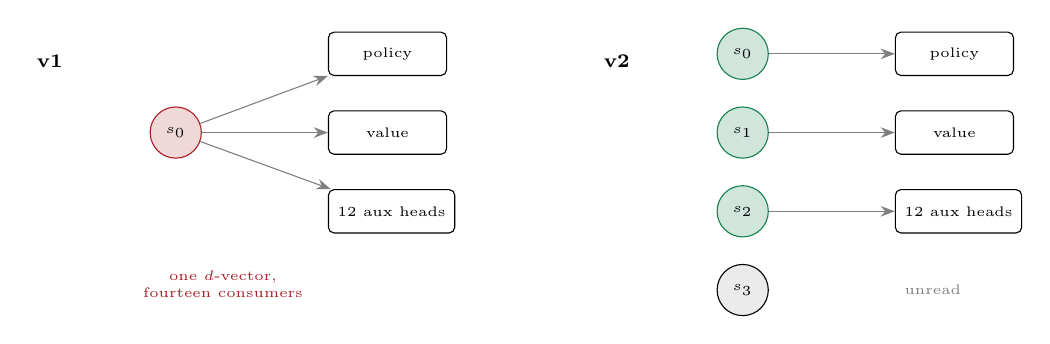
\begin{tikzpicture}[font=\small]
\tikzset{
 s/.style={draw,circle,minimum size=6.5mm,inner sep=0,font=\tiny},
 h/.style={draw,rounded corners=2pt,minimum height=5.5mm,minimum width=15mm,font=\tiny,align=center},
 ar/.style={-{Stealth[length=1.8mm]},gray}
}
\node[font=\scriptsize\bfseries] at (-1.6,0.9) {v1};
\node[s,fill=cBad!18,draw=cBad] (a) at (0,0) {$s_0$};
\node[h,right=16mm of a,yshift=10mm] (p1) {policy};
\node[h,right=16mm of a] (v1) {value};
\node[h,right=16mm of a,yshift=-10mm] (x1) {12 aux heads};
\draw[ar] (a)--(p1); \draw[ar] (a)--(v1); \draw[ar] (a)--(x1);
\node[font=\tiny,text=cBad,below=13mm of a,align=center,xshift=6mm] {one $d$-vector,\\fourteen consumers};

\node[font=\scriptsize\bfseries] at (5.6,0.9) {v2};
\node[s,fill=cV2!20,draw=cV2] (b0) at (7.2,1.0) {$s_0$};
\node[s,fill=cV2!20,draw=cV2] (b1) at (7.2,0.0) {$s_1$};
\node[s,fill=cV2!20,draw=cV2] (b2) at (7.2,-1.0) {$s_2$};
\node[s,fill=black!8] (b3) at (7.2,-2.0) {$s_3$};
\node[h,right=16mm of b0] (p2) {policy};
\node[h,right=16mm of b1] (v2) {value};
\node[h,right=16mm of b2] (x2) {12 aux heads};
\node[font=\tiny,right=16mm of b3,text=gray] {unread};
\draw[ar] (b0)--(p2); \draw[ar] (b1)--(v2); \draw[ar] (b2)--(x2);
\end{tikzpicture}
\caption{Pooling fan-out. v1 routes a single pooled vector to every consumer.
v2 gives the policy, the value head and the auxiliary bank their own seed, so
each consumer's gradient shapes its own read of the board.}
\label{fig:pma}
\end{figure}

\paragraph{Assigning seeds to consumers is a routing choice, and it is the part
without a citation. \tagS}
That $k$ seeds exist is standard; that seed $0$ feeds the policy, seed $1$ the
value head and seed $2$ the auxiliary bank is a design decision specific to this
project. It is well-motivated --- disjoint read-outs mean each seed receives
gradient from exactly one consumer, which forces the specialisation that
otherwise merely has permission to emerge --- but no published result is being
relied on, and none should be cited as if it were.

\paragraph{$k$ seeds give $k$ rank-one reads, not a full-rank read. \tagT}
A single-layer PMA is one softmax-weighted average, i.e.\ a rank-one summary of
the token set; $k$ seeds give $k$ of them. This is a partial answer to the
objection that a pooled read cannot express conjunctions over the board
(``their active is a two-prize threat \emph{and} I have exactly enough energy
\emph{and} they have one prize left''), not a complete one.

\subsection{A structural confound: FiLM and multi-seed pooling cannot be
separated in the current code}
\label{sec:confound}

This is the most consequential implementation finding in this document.

\begin{itemize}\itemsep2pt
\item The constructor \textbf{raises} if \texttt{arch\_v2} is set with fewer than
three pool seeds, because the v2 forward reads seeds $0$, $1$ and $2$ by index.
\item The pooling module is built as $\mathrm{PMA}(d,h,\text{seeds}=k)$ \emph{only}
when \texttt{arch\_v2} is on; under v1 the seed count is ignored and pooling
falls back to a single seed.
\end{itemize}

\noindent
Therefore \texttt{arch\_v2} $\Leftrightarrow$ multi-seed pooling, enforced at
construction. There is no configuration that isolates FiLM from multi-seed
pooling, in either direction. A side effect worth its own note: the v1 arm's
manifest records \texttt{pool\_seeds: 4} while the code ignored the flag and
built a single seed --- a manifest that documents an intent the run did not
execute, which is the same class of defect as a device flag recorded by an
implementation that cannot use it.

\paragraph{What this does and does not invalidate.} It makes the v1-versus-v2
comparison \emph{undecomposable}: FiLM, pooling seeds and standardisation moved
together and no configuration separates the first two, so no per-component
attribution can be drawn from it. It does \emph{not} invalidate single-variable
runs that toggle one flag against a \emph{fixed} v2 baseline --- relations on or
off, head geometry, model width. Those remain attributable to their own
variable; they were never capable of decomposing the v2 package, and should not
be described as if they were. Decoupling the flags is a change to a file that is
frozen while runs import it, so it belongs in the next generation, together with
the per-family $W_f$ cosine test of \S\ref{sec:filmtest}.

\section{Per-column standardisation}

Raw numeric columns span a measured $39{,}570\times$ in per-column standard
deviation; a signed $\log(1+|x|)$ leaves $891\times$; the learned projection's
per-column norms span only $9.27\times$, so the network does \emph{not}
compensate for the residual imbalance. Five of $160$ columns carry half the
input variance entering the projection, while $52$ binary flags --- most of the
hand-engineered feature surface --- carry $2.3\%$. \tagM

\paragraph{The fold is exact. \tagT}
Standardising $x' = (x-\mu)/\sigma$ and absorbing it into an existing checkpoint by
\[
W'_{:,j} = W_{:,j}\,\sigma_j, \qquad b' = b + W\mu
\]
gives $W'x' + b' = W(x-\mu) + b + W\mu = Wx + b$, so the warm start is
bit-identical at initialisation while gradients are equalised from the first
step. Two constraints are load-bearing: $\sigma_j = 0$ must pass through
unchanged rather than divide, and $\sigma$ must be robust (median/IQR with a
floor), because spike distributions are common in this feature set --- a column
that is $0$ on most rows and $40$ on the rest is scaled \emph{into} an outlier by
a naive standard deviation rather than out of one.

\section{The relation that erases what it is for}
\label{sec:reldefect}

Attribute relations are assigned by two successive overwrites: same-owner first,
then same-zone \emph{unconditionally}. Because family and owner are separate
tags, every pair sharing a family receives the same-zone identifier regardless of
owner --- so a bench token and the opposing bench token can carry the identifier
that is supposed to distinguish them. The same logic appears in a second code
path. Measured over 400 real rows, excluding padding: \tagM

\begin{center}
\begin{tabular}{lr}
\toprule
same-owner pairs relabelled to same-zone & $371{,}200/1{,}200{,}682 = 30.92\%$ \\
same-zone pairs that are in fact cross-owner & $13{,}904/385{,}104 = 3.61\%$ \\
\bottomrule
\end{tabular}
\end{center}

\noindent
The defect is real and should be repaired in both code paths. It is
\emph{not}, however, a sufficient explanation for the relational bias being
inert. That bias is a scalar per (relation, head) --- $768$ parameters across all
twelve blocks --- and trains to an absolute maximum of $0.035$ in a logit space
of unit scale, flipping $0.2$--$0.3\%$ of decisions. The instance pointer, which
delivers a relation as a full $d$-dimensional input feature, uses $294{,}912$
parameters and flips $36.2\%$. \tagM\ The honest reading is about
\emph{delivery mechanism}: relations supplied as input features work here;
relations supplied as scalar attention biases do not. A $3.61\%$ mislabelling
rate on one identifier does not account for the gap.

\section{Seed variation, and why single-run comparisons should not be published}
\label{sec:seeds}

There are two seed bands in this project and they are not interchangeable. One
is the spread of \emph{offline top-1} across training seeds; the other is the
spread of \emph{arena win rate} across match seeds. They differ by roughly an
order of magnitude, for the ordinary reason that a win rate over a few hundred
paired matchups is far noisier than an accuracy over fifteen thousand rows. A
band quoted without naming its quantity invites comparison against something
nobody measured.

\begin{center}
\begin{tabular}{lccl}
\toprule
band & quantity & between-seed SD & source \\
\midrule
offline & contested top-1 & $0.15$--$0.27$\,pp & 20 training runs, Fig.~\ref{fig:seeds} \\
arena   & win rate        & $2.51$--$2.52$\,pp & 16 match seeds, Fig.~\ref{fig:arena} \\
\bottomrule
\end{tabular}
\end{center}

\begin{figure}[h]
\centering
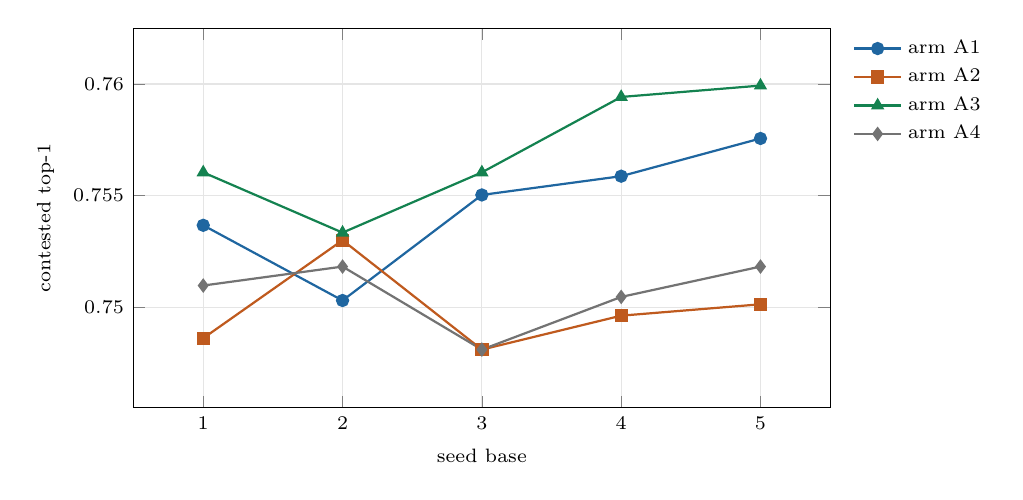
\begin{tikzpicture}
\begin{axis}[
  width=0.86\textwidth, height=6.4cm,
  xlabel={seed base}, ylabel={contested top-1},
  xmin=0.5, xmax=5.5, xtick={1,2,3,4,5},
  ymin=0.7455, ymax=0.7625,
  yticklabel style={/pgf/number format/fixed,/pgf/number format/precision=4},
  legend style={font=\scriptsize,at={(1.02,1)},anchor=north west,draw=none},
  grid=both, grid style={black!10}, tick label style={font=\scriptsize},
  label style={font=\scriptsize},
]
\addplot[mark=*,thick,cState]        coordinates {(1,0.75367)(2,0.75030)(3,0.75503)(4,0.75587)(5,0.75756)};
\addlegendentry{arm A1}
\addplot[mark=square*,thick,cOpt]    coordinates {(1,0.74861)(2,0.75300)(3,0.74810)(4,0.74962)(5,0.75013)};
\addlegendentry{arm A2}
\addplot[mark=triangle*,thick,cV2]   coordinates {(1,0.75604)(2,0.75334)(3,0.75604)(4,0.75942)(5,0.75993)};
\addlegendentry{arm A3}
\addplot[mark=diamond*,thick,black!55]coordinates {(1,0.75097)(2,0.75182)(3,0.74810)(4,0.75046)(5,0.75182)};
\addlegendentry{arm A4}
\end{axis}
\end{tikzpicture}
\caption{Twenty runs: four architecture arms at five seed bases each, scored on
contested top-1 (forced single-option decisions excluded). Between-seed standard
deviation is $0.15$--$0.27$\,pp and the full five-seed range is $0.37$--$0.73$\,pp.
Arm A1 beats arm A2 on the five-seed mean ($0.7545$ against $0.7499$, a
$0.46$\,pp effect) and at four of the five seeds --- but at seed base 2 the
ordering reverses. A comparison run at a single seed therefore returns the
wrong sign on a real effect one draw in five.}
\label{fig:seeds}
\end{figure}

\begin{figure}[h]
\centering
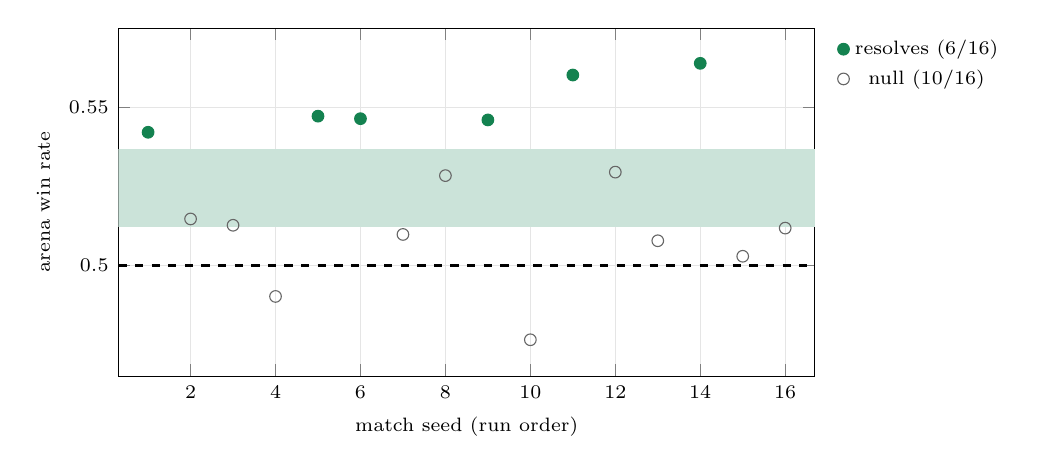
\begin{tikzpicture}
\begin{axis}[
  width=0.86\textwidth, height=6.0cm,
  xlabel={match seed (run order)}, ylabel={arena win rate},
  xmin=0.3, xmax=16.7, xtick={2,4,6,8,10,12,14,16},
  ymin=0.465, ymax=0.575,
  yticklabel style={/pgf/number format/fixed,/pgf/number format/precision=3},
  legend style={font=\scriptsize,at={(1.02,1)},anchor=north west,draw=none},
  grid=both, grid style={black!10}, tick label style={font=\scriptsize},
  label style={font=\scriptsize},
]
\addplot[draw=none,forget plot,name path=lo] coordinates {(0.3,0.5121)(16.7,0.5121)};
\addplot[draw=none,forget plot,name path=hi] coordinates {(0.3,0.5367)(16.7,0.5367)};
\addplot[cV2!22,forget plot] fill between[of=lo and hi];
\addplot[black,dashed,thick,forget plot] coordinates {(0.3,0.5)(16.7,0.5)};
\addplot[only marks,mark=*,mark size=2.1pt,cV2] coordinates
  {(1,0.5421)(5,0.5472)(6,0.5464)(9,0.5460)(11,0.5602)(14,0.5639)};
\addlegendentry{resolves ($6/16$)}
\addplot[only marks,mark=o,mark size=2.1pt,black!60] coordinates
  {(2,0.5147)(3,0.5127)(4,0.4902)(7,0.5098)(8,0.5284)(10,0.4765)(12,0.5295)(13,0.5078)(15,0.5029)(16,0.5118)};
\addlegendentry{null ($10/16$)}
\end{axis}
\end{tikzpicture}
\caption{The same comparison run at sixteen match seeds, $256$ paired matchups
each. Dashed line is no effect; the shaded band is the pooled $95\%$ interval,
$[0.5121, 0.5367]$, which excludes $0.5$. Ten of the sixteen individual runs do
\emph{not} resolve on their own paired interval, and two of them fall below
$0.5$ outright. The effect is real and the median single run fails to find it.}
\label{fig:arena}
\end{figure}

\paragraph{Applying this to the current v1-versus-v2 result.} Both arms were
trained on identical splits ($4{,}920$ train / $868$ validation games;
$19{,}900$ validation rows of which $15{,}804$ are contested), at the record
shape, from the same seed, for two epochs:

\begin{center}
\begin{tabular}{lccc}
\toprule
& contested top-1 & Brier & headline top-1 \\
\midrule
v1 & $0.7281$ & $0.4144$ & $0.7598$ \\
v2 & $0.7371$ & $0.3975$ & $0.7669$ \\
\midrule
$\Delta$ & $\mathbf{+0.90}$\,pp & $-0.0170$ & $+0.71$\,pp \\
\bottomrule
\end{tabular}
\end{center}

\noindent
The margin is larger on contested decisions than on the headline, which is the
right direction: v2 gains where a choice actually exists. \tagM\ \textbf{This
number is provisional pending the paired interval below, and should be cited
that way.} Three qualifications belong beside it, and none of them is optional.

\begin{enumerate}\itemsep2pt
\item \textbf{$n=1$ seed per arm.} The $+0.90$\,pp exceeds the largest five-seed
range we have measured ($0.73$\,pp), which is encouraging, but that band comes
from a different corpus, a different width and head count, and ten epochs rather
than two. Early training is the noisier regime, so the band almost certainly
understates seed noise here. A second seed is the minimum.
\item \textbf{The comparison is paired on data and split but not on
initialisation}, since v2 adds parameters and the random stream diverges.
\item \textbf{The correct test has not been run.} Because both models are scored
on the same games, the statistic that settles this is the per-game difference in
contested accuracy, bootstrapped over the $868$ validation games --- not a
row-level interval, which treats $15{,}804$ correlated rows as independent and is
optimistic by roughly $4\times$ here. This costs one evaluation pass that writes
per-game accuracies.
\end{enumerate}

\paragraph{And the result is a package, not a component.} The v2 arm moved FiLM,
pooling seeds and standardisation together. Per \S\ref{sec:confound}, the first
two cannot be separated at all in the current code. The defensible claim today is
``the v2 package beats v1 by $+0.90$\,pp contested at one seed''; no
per-component attribution is available.

\section{What this architecture does not do}

Stated plainly, because a design document that lists only its strengths hides the
more useful half.

\begin{itemize}\itemsep2pt
\item \textbf{No search and no lookahead at inference.} The policy is evaluated
once per decision. A learned evaluator combined with search is the structural
claim behind AlphaZero \cite{silver2017alphazero}; nothing here exercises it.
\item \textbf{No opponent modelling.} All twelve auxiliary heads describe our own
side. The opponent's threat enters only through the board being visible.
\item \textbf{Cross-turn history is almost absent.} Intra-turn memory exists as
ordinal-indexed tokens, but cross-turn history is a handful of near-empty tokens
carrying a count and a type identifier. Conditioning on action history is
deliberately \emph{not} added: it is refuted for imitation learning by
\cite{dehaan2019causal,wen2020copycat,ortega2021delusions} and by this project's
own removal of it with evidence.
\item \textbf{No positional encoding over tokens}, which would be a category
error on a set.
\item \textbf{Imitation is bounded by its teacher.} Only search or self-play can
exceed that bound, and neither is in the deployed path.
\end{itemize}

\section{Claims withdrawn}

\paragraph{Auxiliary heads are not worth $+45$ ladder points.} That figure
compared a multitask run against a pure-imitation run from a different pipeline.
An audit of every run in this project found that \emph{no} run has ever supplied
an auxiliary target table; six auxiliary heads are constructed from a hardcoded
fallback and have never received a gradient from a label. The comparison does not
transfer and the claim is withdrawn. \tagM

\paragraph{The rejection of FiLM in the ground-up design document does not
follow from its cited evidence.} That document rejects family-conditioned
gain in favour of per-field direction vectors, on the grounds that the two
readings of a shared column are ``unrelated quantities needing different
directions''. The measurement offered ($0.0241$ against $0.0003$) shows one
family not using the column, which is interference and is exactly what a gain
repairs. The rejection may still be right, but not on that evidence, and the
arm that shipped FiLM is currently ahead. \tagM

\paragraph{A between-seed spread of $2.52$\,pp was mislabelled, not unsourced ---
and it reproduces exactly.} The figure is the between-seed standard deviation of
\emph{arena win rate}, not of offline top-1, and it was handed on without naming
its quantity. Recomputed from the raw per-seed artefacts, the first twelve seeds
give mean $0.5253$, SD $0.0252$ ($2.52$\,pp), standard error $0.0073$, $95\%$
interval $[0.5110, 0.5396]$ --- a bit-exact reproduction. Four further seeds have
since landed; at sixteen the estimate is mean $0.5244$, SD $0.0251$, interval
$[0.5121, 0.5367]$, still excluding $0.5$ and slightly tighter. The two bands in
\S\ref{sec:seeds} are both correct and neither substitutes for the other; the
defect was the missing label, which is the same failure as an unlabelled hash. \tagM

\paragraph{The justification given for bootstrapped value targets does not
apply.} The stated reason to prefer temporal-difference targets over regression
is that recorded labels are ``$22\%$ noisy on pair-order replication.'' That
number traces to an eight-sample repeatability audit of seventeen contexts in an
unrelated ranking experiment from an earlier phase of the project --- not to the
recorded terminal labels of the replay corpus. Good reasons to prefer
bootstrapping exist (variance and credit assignment across roughly a hundred
decisions per game); this is not one of them, and it should be struck. \tagM

\section{The corpus has no terminal state}

A finding that constrains any value-function work built on recorded play.
Sampling replays evenly across all forty-five days of the high-Elo corpus: \tagM

\begin{center}
\begin{tabular}{lr}
\toprule
replays containing a match-result log entry & $0/288 = 0.0\%$ \\
last observation with the game marked finished & $0/360 = 0.0\%$ \\
\emph{any} observation with the game marked finished & $0/144 = 0.0\%$ \\
last observation with exactly one seat at zero prizes & $0/360 = 0.0\%$ \\
top-level win/loss reward well-formed & $288/288 = 100\%$ \\
\bottomrule
\end{tabular}
\end{center}

\noindent
The engine emits a terminal reason during live play; the replay serialisation
does not preserve it, because the last recorded observation is the one the agent
was asked to act on. The \emph{outcome} is available and exact; the terminal
\emph{state} is not. Consequently a prize-margin target cannot be read from this
corpus. The tempting substitute --- treating the last observed prize counts as
terminal --- mispredicts the winner $21.4\%$ of the time while passing every
schema, range and completeness check that would normally be applied to it.

\begin{thebibliography}{9}
\bibitem{perez2018film} E.~Perez, F.~Strub, H.~de~Vries, V.~Dumoulin, A.~Courville.
  \emph{FiLM: Visual Reasoning with a General Conditioning Layer.} AAAI 2018.
  \url{https://arxiv.org/abs/1709.07871}
\bibitem{lee2019set} J.~Lee, Y.~Lee, J.~Kim, A.~Kosiorek, S.~Choi, Y.~W.~Teh.
  \emph{Set Transformer: A Framework for Attention-based Permutation-Invariant
  Neural Networks.} ICML 2019. \url{https://arxiv.org/abs/1810.00825}
\bibitem{silver2017alphazero} D.~Silver et al.
  \emph{Mastering Chess and Shogi by Self-Play with a General Reinforcement
  Learning Algorithm.} 2017. \url{https://arxiv.org/abs/1712.01815}
\bibitem{dehaan2019causal} P.~de~Haan, D.~Jayaraman, S.~Levine.
  \emph{Causal Confusion in Imitation Learning.} NeurIPS 2019.
  \url{https://arxiv.org/abs/1905.11979}
\bibitem{wen2020copycat} C.~Wen, J.~Lin, T.~Darrell, D.~Jayaraman, Y.~Gao.
  \emph{Fighting Copycat Agents in Behavioral Cloning from Observation
  Histories.} NeurIPS 2020. \url{https://arxiv.org/abs/2010.14876}
\bibitem{ortega2021delusions} P.~A.~Ortega et al.
  \emph{Shaking the Foundations: Delusions in Sequence Models for Interaction
  and Control.} 2021. \url{https://arxiv.org/abs/2110.10819}
\bibitem{ng1999shaping} A.~Y.~Ng, D.~Harada, S.~Russell.
  \emph{Policy Invariance Under Reward Transformations.} ICML 1999.
\bibitem{guo2017calibration} C.~Guo, G.~Pleiss, Y.~Sun, K.~Q.~Weinberger.
  \emph{On Calibration of Modern Neural Networks.} ICML 2017.
  \url{https://arxiv.org/abs/1706.04599}
\end{thebibliography}

\end{document}
